
\documentclass[nooutcomes]{ximera}
%\documentclass[space,handout,nooutcomes]{ximera}

% For preamble materials

\usepackage{pgf,tikz}
\usepackage{mathrsfs}
\usetikzlibrary{arrows}
\usepackage{framed}
\usepackage{amsmath}
%\pgfplotsset{compat=1.16}

\graphicspath{
  {./}
  {algorithms/}
  {../algorithms/}
}

\pdfOnly{\renewenvironment{image}[1][]{\begin{center}}{\end{center}}}

%%% This set of code is all of our user defined commands
\newcommand{\bysame}{\mbox{\rule{3em}{.4pt}}\,}
\newcommand{\N}{\mathbb N}
\newcommand{\C}{\mathbb C}
\newcommand{\W}{\mathbb W}
\newcommand{\Z}{\mathbb Z}
\newcommand{\Q}{\mathbb Q}
\newcommand{\R}{\mathbb R}
\newcommand{\A}{\mathbb A}
\newcommand{\D}{\mathcal D}
\newcommand{\F}{\mathcal F}
\newcommand{\ph}{\varphi}
\newcommand{\ep}{\varepsilon}
\newcommand{\aph}{\alpha}
\newcommand{\QM}{\begin{center}{\huge\textbf{?}}\end{center}}

\renewcommand{\le}{\leqslant}
\renewcommand{\ge}{\geqslant}
\renewcommand{\a}{\wedge}
\renewcommand{\v}{\vee}
\renewcommand{\l}{\ell}
\newcommand{\mat}{\mathsf}
\renewcommand{\vec}{\mathbf}
\renewcommand{\subset}{\subseteq}
\renewcommand{\supset}{\supseteq}
\renewcommand{\emptyset}{\varnothing}
\newcommand{\xto}{\xrightarrow}
\renewcommand{\qedsymbol}{$\blacksquare$}
\newcommand{\bibname}{References and Further Reading}
\renewcommand{\bar}{\protect\overline}
\renewcommand{\hat}{\protect\widehat}
\renewcommand{\tilde}{\widetilde}
\newcommand{\tri}{\triangle}
\newcommand{\minipad}{\vspace{1ex}}
\newcommand{\leftexp}[2]{{\vphantom{#2}}^{#1}{#2}}

%% More user defined commands
\renewcommand{\epsilon}{\varepsilon}
\renewcommand{\theta}{\vartheta} %% only for kmath
\renewcommand{\l}{\ell}
\renewcommand{\d}{\, d}
\newcommand{\ddx}{\frac{d}{dx}}
\newcommand{\dydx}{\frac{dy}{dx}}


\usepackage{bigstrut}


\newenvironment{sectionOutcomes}{}{}

\usepackage{array}
%\setlength{\extrarowheight}{-.2cm}   % Commented out by Findell to fix table headings.  Was this for typesetting division?  
\newdimen\digitwidth
\settowidth\digitwidth{9}
\def~{\hspace{\digitwidth}}
\def\divrule#1#2{
\noalign{\moveright#1\digitwidth
\vbox{\hrule width#2\digitwidth}}}


\title{Series}
\author{Bart Snapp and Brad Findell and Jenny Sheldon}
\begin{document}
\begin{abstract}
More problems about series.  Mostly geometric. 
\end{abstract}
\maketitle


%\begin{problem}
%Problem
%\begin{freeResponse}
%\begin{hint}
%Hint
%\end{hint}
%\end{freeResponse}
%\end{problem} 

\begin{problem}
A series is the $\answer[format=string]{sum}$ of consecutive terms from a(n) $\answer[format=string]{sequence}$.  

An arithmetic series is the $\answer[format=string]{sum}$ of consecutive terms from a(n) $\answer[format=string]{arithmetic sequence}$.  

A geometric series is the $\answer[format=string]{sum}$ of consecutive terms from a(n) $\answer[format=string]{geometric sequence}$.  
\end{problem}


\begin{problem}
Consider the geometric series: 
\[
\frac{1}{2}+\frac{1}{4}+\frac{1}{8}+\dots+\frac{1}{2048}
\]
First compute the sequence of partial sums: 
\[
\begin{array}{c|c} \hline
\text{No. of terms} & \text{Value} \\ \hline
1 & \answer{\frac{1}{2}} \\
2 & \answer{\frac{3}{4}} \\
3 & \answer{\frac{7}{8}}\\
4 & \answer{\frac{15}{16}}\\
5 & \answer{\frac{31}{32}}\\
6 & \answer{\frac{63}{64}}\\
\end{array}
\]
\begin{problem}
Make a conjecture: The sum of the first $n$ terms of this series is $\answer{1-\frac{1}{2^n}}$. 

In the series
\[
\frac{1}{2}+\frac{1}{4}+\frac{1}{8}+\dots+\frac{1}{2048}
\]
there are $\answer{11}$ terms, so the sum is $\answer{1-\frac{1}{2^{11}}}$.  

\begin{problem}

Here is picture that can help explain why this particular series works out so nicely: 
\begin{image}
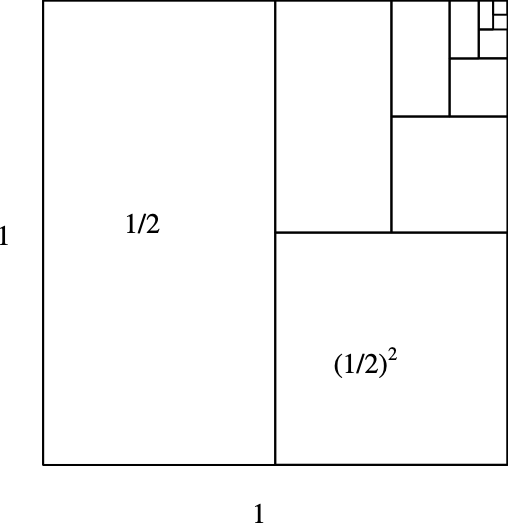
\includegraphics{pbpsqgeo.png}
\end{image}

Begin with a unit square, and then shade an area equal to each term.  At each step in the process, the area remaining unshaded is exactly equal to the area of the region last shaded.  For example, after shading $\frac{1}{2}$ and then $\frac{1}{4}$, $\frac{1}{2}$ remains unshaded.  

Furthermore, it appears that as more and more terms are added, the sum should get closer and closer to $\answer{1}$.  

The following examples provide a general approach for geometric series.  
\end{problem}
\end{problem}
\end{problem}



\end{document}



